\documentclass[tikz,border=8pt]{standalone}
% Shared preamble for the bootqcc TikZ figures.
\usepackage[T1]{fontenc}
\usepackage{helvet}
\renewcommand{\familydefault}{\sfdefault}
\usepackage{amsmath}
\usetikzlibrary{arrows.meta,positioning,shapes.geometric,fit,backgrounds,calc}

\definecolor{navy}{HTML}{1F3A5F}
\definecolor{sky}{HTML}{5AA9E6}
\definecolor{coral}{HTML}{FF6B6B}
\definecolor{slate}{HTML}{6B7A8F}

\tikzset{
  box/.style={rectangle, rounded corners=4pt, draw=navy, fill=sky!15, thick,
              align=center, minimum height=1.0cm, inner sep=6pt, text width=4.6cm},
  inbox/.style={rectangle, rounded corners=4pt, draw=slate, fill=slate!10, thick,
              align=center, minimum height=0.9cm, inner sep=5pt, text width=3.0cm,
              font=\small},
  io/.style={trapezium, trapezium left angle=72, trapezium right angle=108,
             draw=navy, fill=white, thick, align=center, minimum height=1.2cm,
             inner sep=5pt, text width=3.0cm},
  result/.style={rectangle, rounded corners=8pt, draw=coral, fill=coral!10, thick,
              align=center, minimum height=1.0cm, inner sep=6pt, text width=4.0cm},
  term/.style={rectangle, rounded corners=12pt, draw=navy, fill=navy, text=white,
               thick, align=center, minimum height=0.9cm, inner sep=6pt, text width=4.2cm},
  dec/.style={diamond, aspect=2.6, draw=navy, fill=white, thick, align=center,
              inner sep=0pt, text width=2.7cm, font=\small},
  err/.style={rectangle, rounded corners=4pt, draw=coral, fill=coral!15, thick,
              align=center, minimum height=0.9cm, inner sep=6pt, text width=3.2cm},
  arr/.style={-{Latex[length=3mm]}, thick, navy},
  lab/.style={font=\footnotesize\bfseries, text=navy, fill=white, inner sep=1.5pt},
  phase/.style={rounded corners=8pt, draw=navy!45, dashed, thick, inner sep=12pt},
}

\begin{document}
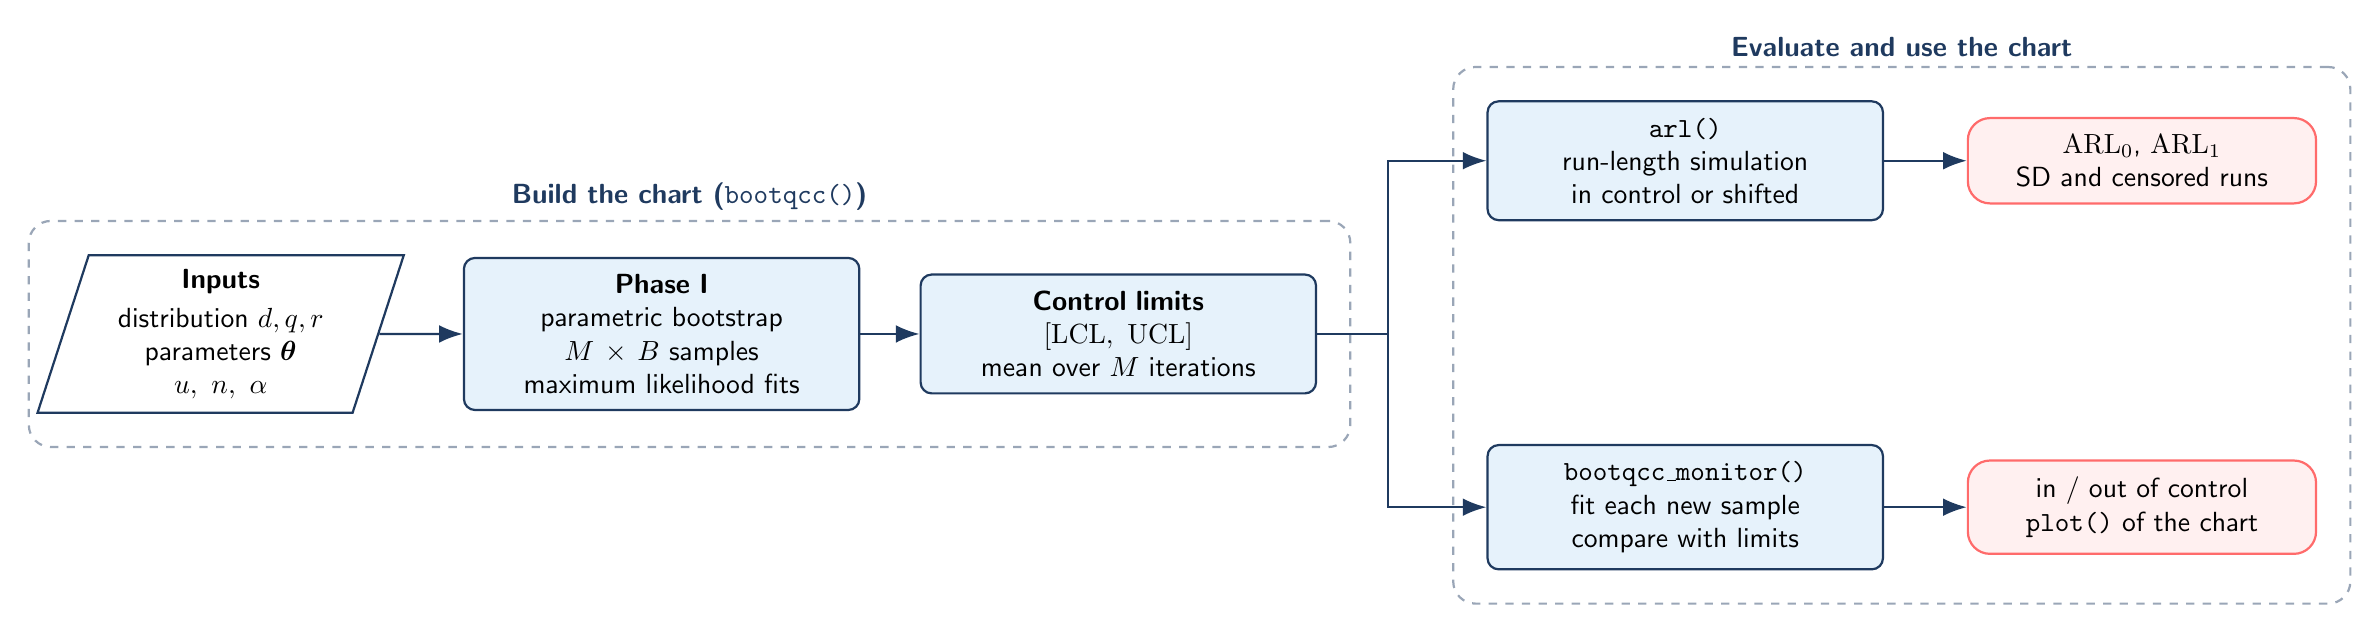
\begin{tikzpicture}[node distance=1cm]

  \node[io]  (inp) at (0,0)
    {\textbf{Inputs}\\[2pt] distribution $d,q,r$\\ parameters $\boldsymbol\theta$\\ $u,\ n,\ \alpha$};
  \node[box] (p1)  at (5.6,0)
    {\textbf{Phase I}\\ parametric bootstrap\\ $M\times B$ samples\\ maximum likelihood fits};
  \node[box] (lim) at (11.4,0)
    {\textbf{Control limits}\\ $[\mathrm{LCL},\ \mathrm{UCL}]$\\ mean over $M$ iterations};

  \node[box] (arl) at (18.6,2.2)
    {\texttt{arl()}\\ run-length simulation\\ in control or shifted};
  \node[box] (mon) at (18.6,-2.2)
    {\texttt{bootqcc\_monitor()}\\ fit each new sample\\ compare with limits};

  \node[result] (arlo) at (24.4,2.2)
    {$\mathrm{ARL}_0$, $\mathrm{ARL}_1$\\ SD and censored runs};
  \node[result] (mono) at (24.4,-2.2)
    {in / out of control\\ \texttt{plot()} of the chart};

  \draw[arr] (inp) -- (p1);
  \draw[arr] (p1)  -- (lim);
  \draw[arr] (lim.east) -- ++(0.9,0) |- (arl.west);
  \draw[arr] (lim.east) -- ++(0.9,0) |- (mon.west);
  \draw[arr] (arl) -- (arlo);
  \draw[arr] (mon) -- (mono);

  \begin{pgfonlayer}{background}
    \node[phase, fit=(inp)(p1)(lim), label={[navy,font=\bfseries]above:Build the chart (\texttt{bootqcc()})}] {};
    \node[phase, fit=(arl)(mon)(arlo)(mono), label={[navy,font=\bfseries]above:Evaluate and use the chart}] {};
  \end{pgfonlayer}
\end{tikzpicture}
\end{document}
